\chapter{Modelling and Simulation}

\graphicspath{{./Figures/Modelling and Simulation}}

In this pivotal chapter, we meticulously derive the center of gravity and the moment of inertia for the two-wheeled self-balancing robot.
These parameters are the linchpins of our dynamic analysis, serving as the critical variables within the equations of motion that govern the robot's behavior.
By calculating these values with precision, we can substitute them into our dynamic equations, thereby tailoring the model to reflect the true dynamics of the robot.
This process not only enhances the accuracy of our simulations but also ensures that the control strategies developed are based on a robust and representative model of the robot's physical capabilities.
The careful derivation of these parameters is a testament to the thoroughness of our approach, ensuring that the resulting model is both reliable and predictive of the robot's real-world performance.
\newpage

\section{Mathematical Modelling}

%	\item \textbf{TWIPR Model:} Explanation of the Two-Wheeled Inverted Pendulum Robot (TWIPR) model.
The two-wheeled Inverted Pendulum robot model is as shown in the figure  \ref{fig:New model} where it consists of two legs that include a hip and knee joints as well as wheels at the end of each leg.
The robot needs to constantly adjust its posture to be able to maintain the balance, just like how the human being balances when standing on the feet.
This new TWIPR model is the latest iteration in the evolution of its predecessor.

%Two subfigures side by side of the two models 	the old model and the new model
\begin{figure}[h]
	\centering
	\begin{subfigure}[t]{0.45\textwidth}
		\centering
		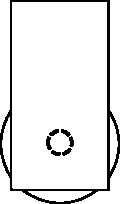
\includegraphics[height=0.7\textwidth]{Old model}
		\caption{Old model}
		\label{fig:Old model}
	\end{subfigure}
	\begin{subfigure}[t]{0.45\textwidth}
		\centering
		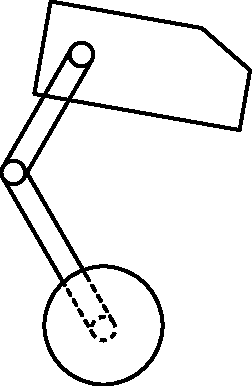
\includegraphics[height=0.7\textwidth]{New model}
		\caption{New model}
		\label{fig:New model}
	\end{subfigure}
	\caption{Comparison between the old and new models}
	\label{fig:Comparison between the old and new models}
\end{figure}

%	\item \textbf{Focus on 2D Dynamics:} Discussion on the scope limited to 2D dynamics and plans for future expansion to 3D dynamics and controller synthesis.
\subsection{2D Dynamics}
%golbal coordinate system and local coordinate system
The scope of this project is limited to 2D dynamics.
However, the model can be extended to 3D dynamics and controller synthesis for the 3D dynamics in the future.
The 2D dynamics is considered for simplification purposes and to reduce the complexity of the model.
The 2D dynamics modeling takes into account the robot's movement in the x-y plane and the rotation of the knee joint, hip joint, and the wheels around the z-axis.
The 2D dynamics modeling considers one leg and half of the body mass.
The other leg and the other half of the mass are symmetrical to the first leg and the first half of the body.
%	\item \textbf{Assumptions and Parameters:} Detailing assumptions such as considering motor angles as parameters.
	%the cansilation of the radial forces and the assumption of the motor angles as parameters.




%	\item \textbf{Model Derivation for \textit{l\_cg} and \textit{I\_y}:} Derivation of the models for center of gravity length (\textit{l\_cg}) and inertia around the y-axis (\textit{I\_y}).
%skip one page

\newpage
%Center of Gravity
\subsection{Center of Gravity }
%	$\bullet$ in that section the calculations of the overall center of gravity
%
%	$\bullet$ Significance in Dynamics:The stability of an object is directly impacted by the COG position, which also affects how it reacts to forces and moments from the outside world.
%
%	$\bullet$ Maintain equilibrium,
%
%	$\bullet$ accurately determining the COG is crucial for predicting and controlling dynamic behavior
%
%	in the above figure in order to simplify the deriviation of the center of
	\begin{figure}[h]
		\centering
		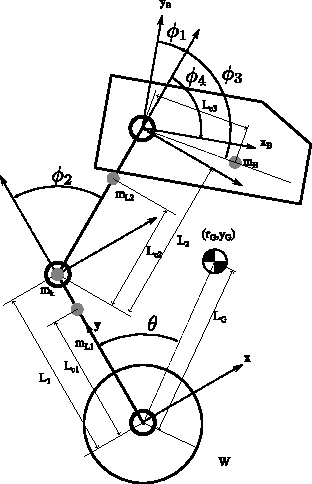
\includegraphics[width=.5\textwidth]{Model}
		\caption[Mechanical model with the local coordinate system]{Figure illustrating the mechanical model with the local coordinate system to determine the center of gravity.}
		\label{fig:Mechanical model with the local coordinate system}
	\end{figure}

The calculation of the center of gravity is crucial for the dynamic analysis of the robot.
The center of gravity is calculated by taking into account the weights of the links, the knee joint, the body and the distances between these weights and the local coordinate system of the robot.
The stability of the robot is directly impacted by the center of gravity position, which also affects how it reacts to forces and moments from the outside world.
The following equations are used to calculate the center of gravity location referencing the local coordinate system of the robot as shown in the figure \ref{fig:Mechanical model with the local coordinate system}.
% input the model figure from the graphics path


	\begin{equation}
		\begin{aligned}
			x_{CG} = \frac{m_{L1} \cdot 0 + m_K \cdot 0 + m_{L2} \cdot L_{C2} \cdot \sin(\phi_2) + m_B \cdot (L_2 \cdot \sin(\phi_2) + L_{C3} \cdot \sin(\phi_2 + \phi_3))}{m_{L1} + m_{L2} + m_K + m_B}
		\end{aligned}
	\end{equation}
Where $x_{CG}$ is the center of gravity in the x-axis.

	\begin{equation}
		\begin{aligned}
			y_{CG} = \frac{m_{L1} \cdot L_{C1} + m_K \cdot L_1 + m_{L2} \cdot (L_1 + L_{C2} \cdot \cos(\phi_2)) + m_B \cdot (L_1 + L_2 \cdot \cos(\phi_2) + L_{C3} \cdot \cos(\phi_2 + \phi_3))}{m_{L1} + m_{L2} + m_K + m_B}
		\end{aligned}
	\end{equation}
Where $y_{CG}$ is the center of gravity in the y-axis.

%expain the equations in more details
	\begin{equation}
		L_G = \sqrt{x_{CG}^2 + y_{CG}^2}
	\end{equation}
The distance between the center of gravity and the Wheel Joint is calculated using the Pythagorean theorem.

	\begin{equation}
		\theta = \arctan\left(\frac{{x_{CG}}}{{y_{CG}}}\right)
	\end{equation}
The angle between the center of gravity $L_G$ and the knee wheel link $L_1$ is calculated using the arctangent function.

\subsection{Moment of inertia}
	\begin{figure}[h]
		\centering
		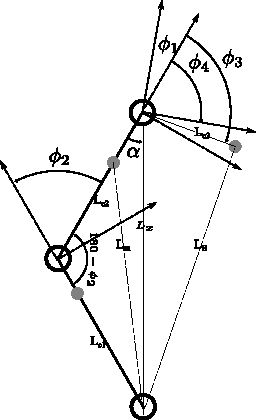
\includegraphics[width=.5\textwidth]{Angles}
		\caption[Moment of inertia Schematic representation]{Schematic representation detailing the requisite angles and lengths for calculating the moment of inertia.}
		\label{fig:Schematic representation xxxxx detailing the requisite angles and lengths for calculating the moment of inertia.}
	\end{figure}


	%MOI
	Moment of inertia calculations are important for the dynamic analysis of the robot. In order to calculate the moment of inertia, the lengths from the wheel joint to the center of mass of each link are calculated. The moment of inertia is calculated using the following equations.
	\begin{equation}
		L_m = \sqrt{L_1^2 + L_{C2}^2 - L_1 L_{C2} \cos(180 - \phi_2)}
	\end{equation}
Where $L_m$ is the distance between the wheel joint and the center of mass of the knee wheel link.
	\begin{equation}
		L_{x} = \sqrt{L_1^2 + L_2^2 - L_1 L_2 \cos(180 - \phi_2)}
	\end{equation}


	\begin{equation}
		\alpha = \cos^{-1} \left( \frac{l_2^2 + l_{x}^2 - l_1^2}{2 l_2 l_{x}} \right)
	\end{equation}

	%explain the equations in more details

	\begin{equation}
		L_b = \sqrt{L_{x}^2 + L_{C3}^2 - Lx L_{C3} \cos(180 - \alpha - \phi_3 )}
	\end{equation}

	\begin{equation}
		I_{L1} = \frac{1}{12} m_{L1} (a_1^2 + b_1^2)
	\end{equation}
	\begin{equation}
		I_{L2} = \frac{1}{12} m_{L2} (a_2^2 + b_2^2)
	\end{equation}
	\begin{equation}
		I_B = \frac{1}{12} m_B (a_B^2 + b_B^2)
	\end{equation}
Since the knee wheel link, the hip knee link and the body are assumed to be cuboids, the moment of inertia of each link is calculated using the equation above.
	\begin{equation}
		I_K = \frac{1}{2} m_K R_m^2
	\end{equation}
	The moment of inertia of the knee joint is calculated using the equation above where the knee joint is assumed to be a cylinder.
	\begin{equation}
		I = I_{L1} + m_{L1} L_{C1}^2 + I_K + m_K L_1^2 + I_{L2} + m_{L2} L_m^2 + I_B + m_B L_b^2
	\end{equation}
	The total moment of inertia of the robot is calculated using the equation above.
%	\item \textbf{Integration into TWIPR Model:} Integration of derived models into a new TWIPR framework.

%	\item \textbf{Linear Model Derivation:} Derivation of the linear model from the integrated TWIPR model.

%	\item Modeling allows for predictive analysis and understanding of the robot's behavior.
	In order to predict the behavior of the robot under different settings, the modeling procedure entails constructing mathematical representations of the robot's dynamics and control systems.
%\end{itemize}







	\newpage
\subsection{Assumptions and Parameters}
Many assumptions as outlined in \ref{tab:parameters} for the figure \ref{fig:Mechanical model with the local coordinate system} were made to simplify the model and reduce the complexity of the calculations. The weights and the lengths of the links are constant, and the angles $\phi_2$, $\phi_3$ are input variables that can be controlled to adjust the robot's posture.
%table of the assumptions
	\begin{table}[h!]
		\centering
		\caption{Parameters of the mechanical system}
		\label{tab:parameters}
		\begin{tabular}{lcl}
			\toprule
			Parameter & Value & Description \\
			\midrule
			$L_1$ & 0.017 m & Length of the Wheel knee Link \\
			$L_2$ & 0.017 m & Length of the Body knee Link \\
			$L_{C1}$ & 0.013 m & Distance between the Wheel Joint and the center of mass of the Wheel knee Link \\
			$L_{C2}$ & 0.013 m & Distance between the Knee Joint and the center of mass of the Body knee Link \\
			$L_{C3}$ & 0.01 m & Distance between the Hip Joint and the center of mass of the body \\
			$m_{L1}$ & 0.2 kg & Mass of the Wheel knee Link \\
			$m_{L2}$ & 0.2 kg & Mass of the Body knee Link \\
			$m_K$ & 0.2 kg & Mass of the Knee Joint \\
			$m_B$ & 0.5 kg & Mass of the Body \\
			$L_G$ & - & Distance between the center of gravity and the Wheel Joint \\
			$\theta$ & - & Angle between the center of gravity and the Wheel knee Link \\
			$\phi_1$ & - & Angle between the Body knee Link and the $y_B$ vertical axis of the body \\
			$\phi_2$ & - & Angle between the Wheel knee Link and the Body knee Link \\
			$\phi_3$ & - & Angle between the Body knee Link and the center of mass of the body \\
			$\phi_4$ & - & Angle between the Body knee Link and the $X_B$ horizontal axis of the body \\
			$L_m$ & - & Distance between the Wheel Joint and the center of mass of the Wheel knee Link \\
			$L_x$ & - & Distance between the Wheel Joint and the center of mass of the hip knee Link \\
			$L_b$ & - & Distance between the Wheel Joint and the center of mass of the body \\
			$\alpha$ & - & Angle between $L_x$ and $L_2$ \\
			$I_{L1}$ & - & Moment of inertia of the knee wheel link around the z-axis \\
			$I_{L2}$ & - & Moment of inertia of the hip knee link around the z-axis \\
			$I_K$ & - & Moment of inertia of the knee joint around the z-axis \\
			$I_B$ & - & Moment of inertia of the body around the z-axis \\
			$I$ & - & Total moment of inertia of the robot around the z-axis \\
			$a_1$ & - & Length of the knee wheel link \\
			$b_1$ & - & Width of the knee wheel link \\
			$a_2$ & - & Length of the hip knee link \\
			$b_2$ & - & Width of the hip knee link \\
			$a_B$ & - & Length of the body \\
			$b_B$ & - & Width of the body \\
			$R_m$ & - & Radius of the knee joint \\
			$a_B$ & - & Length of the body \\
			$b_B$ & - & Width of the body \\
			\bottomrule
		\end{tabular}
	\end{table}
	\newpage
	\subsection{Dynamics of the Two-Wheeled Inverted Pendulum Robot}
%figure of the TWIPR dynamics
	\begin{figure}[h]
		\centering
		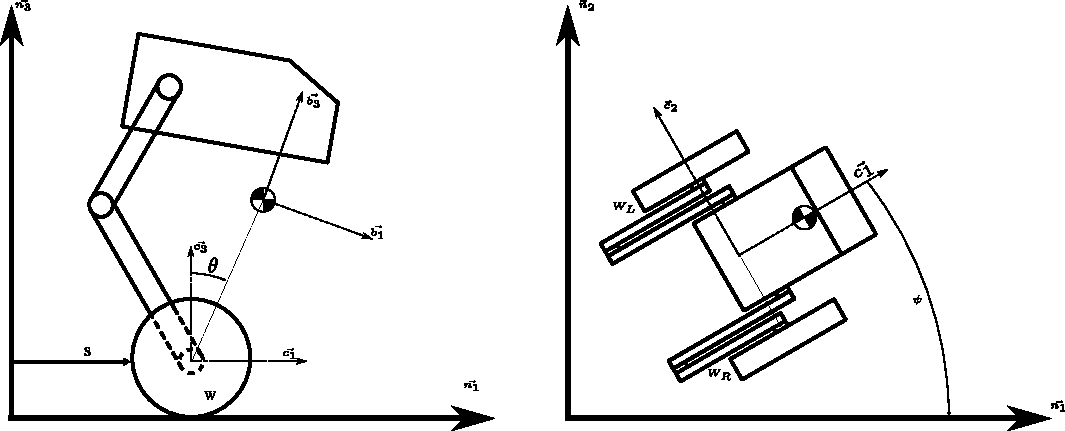
\includegraphics[width=1\textwidth]{TWIPR dynamics}
		\caption[Two-Wheeled Inverted Pendulum Robot Dynamics]{Figure illustrating the Two-Wheeled Inverted Pendulum Robot Dynamics.}
		\label{fig:Two-Wheeled Inverted Pendulum Robot Dynamics}
	\end{figure}

	Given the functions $B_i: \mathbb{R} \rightarrow \mathbb{R}$, $C_{ij}: \mathbb{R} \rightarrow \mathbb{R}$, $D_{ij}: \mathbb{R} \rightarrow \mathbb{R}$, and $V_i: \mathbb{R} \rightarrow \mathbb{R}$, $i,j \in \{1,2,3\}$, the equations of motion are given by:

	\begin{align}
		\ddot{s} &= \frac{\sin(\theta)}{V_1(\theta)} \left( -C_{11}(\theta)g + C_{12}\dot{\theta}^2 + C_{13}(\theta)\dot{\psi}^2 \right) - \frac{D_{11}(\theta)}{V_1(\theta)}\dot{s} + \frac{D_{12}(\theta)}{V_1(\theta)}\dot{\theta} + \frac{B_{1}(\theta)}{V_1(\theta)}(\tau_L + \tau_R) \\
		\ddot{\theta} &= \frac{\sin(\theta)}{V_1(\theta)} \left( C_{21} - C_{22}(\theta)\dot{\theta}^2 - C_{23}(\theta)\dot{\psi}^2 \right) + \frac{D_{21}(\theta)}{V_1(\theta)}\dot{s} - \frac{D_{22}(\theta)}{V_1(\theta)}\dot{\theta} - \frac{B_{2}(\theta)}{V_1(\theta)}(\tau_L + \tau_R)  \\
		\ddot{\psi} &= \frac{\sin(\theta)}{V_2(\theta)} \left( C_{31}(\theta)\dot{\theta}\dot{\psi} - C_{32}(\theta)\dot{\psi}\dot{s} \right) - \frac{D_{33}(\theta)}{V_2(\theta)}\dot{\psi} - \frac{B_{3}}{V_2(\theta)}(\tau_L - \tau_R)
	\end{align}


	The equations of motion are derived in \cite{kim2015dynamic}. The functions $B_i: \mathbb{R} \rightarrow \mathbb{R}$, $C_{ij}: \mathbb{R} \rightarrow \mathbb{R}$, $D_{ij}: \mathbb{R} \rightarrow \mathbb{R}$, and $V_i: \mathbb{R} \rightarrow \mathbb{R}$, $i,j \in \{1,2,3\}$, are given by:

	\begin{equation}
		C_{11}(\theta) = m_B^2 l^2 \cos(\theta)g,
	\end{equation}
	\begin{equation}
		C_{12} = (I_2 + m_B l^2) m_B l,
	\end{equation}
	\begin{equation}
		C_{13}(\theta) = (I_2 + m_B l^2) m_B l + m_B l (I_3 - I_1 - m_B l^2) \cos^2(\theta),
	\end{equation}
	\begin{equation}
		C_{21} = (m_B + 2m_W + \frac{2J}{r^2}) m_B l,
	\end{equation}
	\begin{equation}
		C_{22}(\theta) = m_B^2 l^2 \cos(\theta),
	\end{equation}
	\begin{equation}
		C_{23}(\theta) = (m_B^2 l^2 + (m_B + 2m_W + \frac{2J}{r^2}) (I_3 - I_1 - m_B l^2) )\cos(\theta).
	\end{equation}
	\begin{equation}
		C_{31}(\theta) = 2 (I_3 - I_1 - m_Bl^2) \cos(\theta),
	\end{equation}
	\begin{equation}
		C_{31}(\theta)  = m_B l,
	\end{equation}
	\begin{equation}
		D_{11}(\theta) = \frac{(I_2 + m_Bl^2) 2c_\alpha}{r^2} - \frac{m_B l \cos(\theta) 2c_\alpha}{r},
	\end{equation}
	\begin{equation}
		D_{12}(\theta) = \frac{(I_2 + m_Bl^2) 2c_\alpha}{r} - 2m_B l \cos(\theta) c_\alpha,
	\end{equation}
	\begin{equation}
		D_{21}(\theta) = \frac{(m_B + 2m_W + \frac{2J}{r^2}) 2c_\alpha}{r} + \frac{m_B l \cos(\theta) 2c_\alpha}{r^2},
	\end{equation}
	\begin{equation}
		D_{22}(\theta) = \frac{(m_B + 2m_W + \frac{2J}{r}) 2c_\alpha + m_B l \cos(\theta) 2c_\alpha}{r},
	\end{equation}
	\begin{equation}
		D_{33}(\theta) = \frac{d^2 c_\alpha}{2r^2 },
	\end{equation}
	\begin{equation}
		B_{1} = (I_2 + m_Bl^2) \frac{1}{r} + m_B l \cos(\theta),
	\end{equation}
	\begin{equation}
		B_{2} = \frac{m_B l \cos(\theta)}{r} + m_B + 2m_W + \frac{2J}{r^2},
	\end{equation}
	\begin{equation}
		B_{3} = \frac{d}{2r},
	\end{equation}
	\begin{equation}
		V_{1} = (m_B + 2m_W + \frac{2J}{r^2}) (I_2 + m_Bl^2) - m_B^2l^2 \cos^2(\theta),
	\end{equation}
	\begin{equation}
		V_{2} = I_3 + 2K + (m_W + \frac{J}{r^2}) \frac{d^2}{2} - (I_3 - I_1 - m_Bl^2) \sin^2(\theta).
	\end{equation}

The functions $B_i: \mathbb{R} \rightarrow \mathbb{R}$, $C_{ij}: \mathbb{R} \rightarrow \mathbb{R}$, $D_{ij}: \mathbb{R} \rightarrow \mathbb{R}$, and $V_i: \mathbb{R} \rightarrow \mathbb{R}$, $i,j \in \{1,2,3\}$, depends on the parameters in table \ref{tab:parameters}.
	\begin{table}[h]
		\centering
		\caption{Parameters of the mechanical system}
		\label{tab:parameters}
		\begin{tabular}{lcl}
			\toprule
			Parameter & Value & Description \\
			\midrule
			$m_B$ & 0.5 kg & mass of the pendulum body \\
			$m_W$ & 0.636 kg & mass of a wheel \\
			$l$ & - & distance between the wheel axis and the pendulum's center of gravity \\
			$d$ & - & distance between the two wheels \\
			$J$ & \(5.175 e^{-4}\) kgm\textsuperscript{2} & moment of inertia of a wheel w.r.t. Reference frame \{C\} in direction of \(c_2\) \\
			$K$ & - & moment of inertia of a wheel w.r.t. reference frame \{C\} in direction of \(c_3\) \\
			$I_1$ & - & moment of inertia of pendulum's body w.r.t. Reference frame \{B\} in direction of \(b_1\) \\
			$I_2$ & - & moment of inertia of pendulum's body w.r.t. Reference frame \{B\} in direction of \(b_2\) \\
			$I_3$ & - & moment of inertia of pendulum's body w.r.t. Reference frame \{B\} in direction of \(b_3\) \\
			$c_\alpha$ & \(4.630 e^{-4}\) Nms & viscous friction coefficient \\
			\bottomrule
		\end{tabular}
	\end{table}
	
	

\subsection{Linearization of the Two-Wheeled Inverted Pendulum Robot}
In this section, we linearize the equations of motion of the legged TWIPR robot about the upright equilibrium point. Movement of the robot is restricted to the x-y plane.

The torque inputs are $\tau_L$ and $\tau_R$ for the left and right wheels, respectively.
%equation tau_L and tau_R are equal
\begin{equation}
	\tau_L = \tau_R = \tau
\end{equation}
%the combined torque input u is equal to the torque tau_L plus tau_R
the sum of the torques $\tau_L$ and $\tau_R$ is equal to the combined torque input $u$ which is an input and a variable.
\begin{equation}
	u = \tau_L + \tau_R = 2\tau
\end{equation}
The degree of freedom for the rotation around the z-axis $\psi$ is eleinated by assuming that the robot is always moving in the x-y plane in a straight line. therfore the equation of motion would be as follows:
\begin{equation}
	\ddot{s} = \frac{\sin(\theta)}{V_1(\theta)} \left( -C_{11}(\theta)g + C_{12}\dot{\theta}^2 \right) - \frac{D_{11}(\theta)}{V_1(\theta)}\dot{s} + \frac{D_{12}(\theta)}{V_1(\theta)}\dot{\theta} + \frac{B_{1}(\theta)}{V_1(\theta)}u
\end{equation}
\begin{equation}
	\ddot{\theta} = \frac{\sin(\theta)}{V_1(\theta)} \left( C_{21} - C_{22}(\theta)\dot{\theta}^2 \right) + \frac{D_{21}(\theta)}{V_1(\theta)}\dot{s} - \frac{D_{22}(\theta)}{V_1(\theta)}\dot{\theta} - \frac{B_{2}(\theta)}{V_1(\theta)}u
\end{equation}
Therefore the state vector would be as follows:
\begin{equation}
	x = \begin{bmatrix}
		\theta \\
		\dot{\theta}\\
		s \\
		\dot{s}
	\end{bmatrix}
\end{equation}

%Using thr functions
\begin{equation}
	f_1(x) = \frac{\sin(\theta)}{V_1(\theta)} \left( C_{21} - C_{22}(\theta)\dot{\theta}^2 \right) + \frac{D_{21}(\theta)}{V_1(\theta)}\dot{s} - \frac{D_{22}(\theta)}{V_1(\theta)}\dot{\theta}
\end{equation}
\begin{equation}
	f_2(x) = \frac{\sin(\theta)}{V_1(\theta)} \left( -C_{11}(\theta)g + C_{12}\dot{\theta}^2 \right) - \frac{D_{11}(\theta)}{V_1(\theta)}\dot{s} + \frac{D_{12}(\theta)}{V_1(\theta)}\dot{\theta}
\end{equation}
\begin{equation}
	g_1(x,u) = \frac{B_{2}(\theta)}{V_1(\theta)}u
\end{equation}
\begin{equation}
	g_2(x,u) = \frac{B_{1}(\theta)}{V_1(\theta)}u
\end{equation}
The system can be represented in the following form:
\begin{equation}
	\dot{x} = \begin{bmatrix}
		x_2 \\
		f_1(x) \\
		x_4    \\
		f_2(x)
	\end{bmatrix} + \begin{bmatrix}
		0 \\
		g_1(x,u) \\
		0 \\
		g_2(x,u)
	\end{bmatrix}
\end{equation}

Linearization at the point $x = 0$, which corresponds to the upright equilibrium of the inverted pendulum, simplifies the system's dynamics as follows:
\begin{equation}
\dot{x} = A_cx + B_cu,
\end{equation}
where $A_c \in \mathbb{R}^{4\times4}$ is the system matrix of the time-continuous system, and $B_c \in \mathbb{R}^{4\times1}$ is the input matrix of the time-continuous system. Discretization of the system with a sampling frequency of 50 hertz yields:
\begin{equation}
x_{k+1} = Ax_k + Bu_k,
\end{equation}
where $k \in \mathbb{N}$ indexes the discrete time steps, $x_k \in \mathbb{R}^4$ denotes the state vector at the $k$-th sample, $u_k \in \mathbb{R}$ denotes the input at the $k$-th sample, $A \in \mathbb{R}^{4\times4}$ is the system matrix of the time-discrete system, and $B \in \mathbb{R}^{4\times1}$ is the input matrix of the time-discrete system \cite{MastersThesis}.



\section{Numerical Simulation}
%\begin{itemize}
%	\item \textbf{Discrete Numerical Simulation:} Elaboration on the process of discrete numerical simulation, including the discrete double integration method to arrive in the state vector.
%\end{itemize}
The discrete numerical simulation is a computational method that is used to model the behavior of dynamic systems over discrete periods of time intervals. In contrast to the continuous numerical simulation, the discrete numerical simulation that typically uses the Euler method to solve the differential equations analytically or working with infinitesimally small-timescale numerical solvers.
\subsection{Discrete numerical simulation}
Discrete numerical simulations approximate the state of the system step by step and evaluate the behavior of the system at predetermined intervals. When an analytical solution is not feasible or real-time simulation is required due to the complexity of the system, this approach is particularly helpful.
\subsection{Discrete double integration method}
The discrete double integration method is used to calculate the state vector of the system at each time step. The state vector is calculated by integrating the acceleration twice to get the position and velocity. The state vector is calculated using the following equation:
\begin{equation}
	x_{k+1} = x_k + \dot{x_k} \Delta t + \frac{1}{2} \ddot{x_k} \Delta t^2
\end{equation}
where $x_k$ is the state vector at the $k$-th sample, $\dot{x_k}$ is the derivative of the state vector at the $k$-th sample, $\ddot{x_k}$ is the second derivative of the state vector at the $k$-th sample, and $\Delta t$ is the time step.


\section{Simulation Environment}
%figure of the block diagram of the simulation environment
\begin{figure}[h]
	\centering
	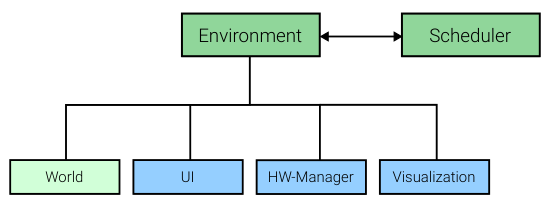
\includegraphics[width=.5\textwidth]{Block Diagram of Simulation Environment}
	\caption{ The environment consists always of a world entity, other parts like user in-
terface(UI), HW-manager and visualization are optional, it is closely linked to
the Scheduler \cite{Bachlorsthesis}}
	\label{fig:Block diagram of the simulation environment}
\end{figure}
The simulation environment is a software framework that is used to simulate the dynamics of the robot. The simulation enviroment is a A complex virtual environment created for realistic testing is the simulation environment. It comprises a variety of spaces with distinct states, dimensions, and mapping capabilities that enable the creation of a wide range of scenarios \cite{Bachlorsthesis}.
\subsection{Physics and Object Primitives}
The simulation ensures realistic movements and interactions by incorporating intricate physics. It makes use of object primitives such as spheres, cylinders, and cuboids, which serve as a basis for building a variety of structures and objects\cite{Bachlorsthesis}.
\subsection{Collision Checking and Dynamics}
The simulation uses sophisticated collision checking techniques, such as pre-checking and distinct algorithms for various situations, such as collisions involving cuboids. To simulate realistic physical interactions between objects, this feature is essential\cite{Bachlorsthesis}.
\subsection{Objects and Agents}
A range of objects, both static and dynamic, including agents that imitate autonomous behavior, are present in the environment. This variety improves the simulation's ability to mimic interactions in the real world.
\subsection{Scheduling and Real Robot Integration}
An advanced scheduling system controls the order and timing of events. Furthermore, the simulation incorporates real robots in a unique way, combining virtual and physical components for thorough testing\cite{Bachlorsthesis}.
\subsection{Integration of the Model}
%figure of the simulation environment
\begin{figure}[h]
	\centering
	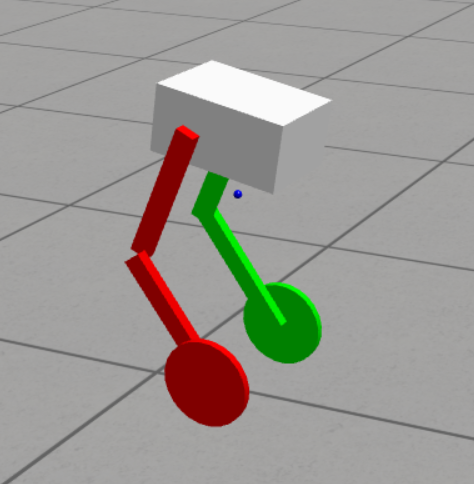
\includegraphics[width=.5\textwidth]{Simulation Environment}
	\caption{The simulation environment}
	\label{fig:The simulation environment}
\end{figure}
As shown in the figure \ref{fig:The simulation environment}, the simulation environment simulates the dynamics of the robot and the controller. where the blue sphere represents the robot center of gravity which changes its location according to the robot's dynamics.



%\begin{itemize}
%	\item \textbf{Overview of the Simulation Environment:} A brief overview of the simulation environment, referencing David's Bachelor Thesis for details.
%
%
%	\item \textbf{Integration of the Model:} Description of integrating the new TWIPR model into the simulation environment and a summary of the individual components of the model.
%\end{itemize}

\section{Controller Synthesis}
%\begin{itemize}
%	\item \textbf{State-Space Controllers:} Introduction to two state-space controllers: Linear Quadratic Regulator (LQR) and Pole-Placement.

%figure of the state space controller
\begin{figure}[h]
	\centering
	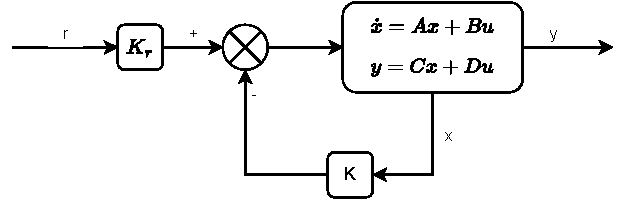
\includegraphics[width=.5\textwidth]{Block Diagram of State Feedback Controller}
	\caption{Block diagram of a state feedback controller}
	\label{fig:Block diagram of a state feedback controller}
\end{figure}


In the realm of modern control theory, State-Space controllers are a pivotal component for managing the behavior of complex systems.Among the most prominent of these controllers are the Linear Quadratic Regulator (LQR) and Pole-Placement controllers, both of which are robust and effective in various applications.
This section provides an overview of these controllers and their application to the legged TWIPR robot.
%full state feedback controllers

\subsection{Linear Quadratic Regulator (LQR)}
The Linear Quadratic Regulator (LQR) is a state-space controller that uses a quadratic cost function to determine the optimal control input for a given system. It aims to minimize the cost function by adjusting the control input, thereby ensuring that the system's state converges to the desired state. The LQR controller is defined by the following equation:
\begin{equation}
	u(t) = -Kx(t)
\end{equation}
where $u(t)$ is the control input, $x(t)$ is the state vector, and $K$ is the gain matrix. The gain matrix is calculated using the following equation:
\begin{equation}
	K = R^{-1}B^TP
\end{equation}
where $R$ is the control weight matrix, $B$ is the input matrix, and $P$ is the solution to the Riccati equation:
\begin{equation}
	A^TP + PA - PBR^{-1}B^TP + Q = 0
\end{equation}
where $A$ is the state matrix and $Q$ is the state weight matrix. The state matrix, state weight matrix, and control weight matrix are defined as follows:
%A = [ 0.5403, -0.8415; 0.8415,  0.5403];
%\begin{equation}
%	A = \begin{bmatrix}
%		0.5403 & -0.8415 \\
%		0.8415 & 0.5403
%	\end{bmatrix}
%\end{equation}
\begin{equation}
	Q = \begin{bmatrix}
		1 & 0 \\
		0 & 1

	\end{bmatrix}
\end{equation}
\begin{equation}
	R = \begin{bmatrix}
		1
	\end{bmatrix}
\end{equation}
The LQR controller is implemented in the simulation environment using the \textit{Python Control Systems Library} \cite{python_control2021}.

\subsection{Pole-Placement Technique}
The Pole-Placement technique is a state-space controller that uses the Ackermann formula to determine the optimal control input for a given system. It aims to place the poles of the system at the desired locations by adjusting the control input, thereby ensuring that the system's state converges to the desired state.placing the poles is not initiutive for high order systems or systems with multiple actuators. The Pole-Placement controller is defined by the following equation:
\begin{equation}
	u(t) = -Kx(t)
\end{equation}
where $u(t)$ is the control input, $x(t)$ is the state vector, and $K$ is the gain matrix. The gain matrix is calculated using the following equation:
\begin{equation}
	K = \begin{bmatrix}
		k_1 & k_2 & k_3
	\end{bmatrix}
\end{equation}
where $k_1$, $k_2$, and $k_3$ are the gains for the first, second, and third states, respectively. The gains are calculated using the following equation:
\begin{equation}
	k_i = \frac{1}{b_i} \left( \sum_{j=0}^{n-1} a_{n-j} \alpha_{i+j} - \alpha_i \right)
\end{equation}
where $a_i$ is the coefficient of the characteristic polynomial, $b_i$ is the coefficient of the denominator polynomial, and $\alpha_i$ is the desired location of the $i$th pole. The characteristic polynomial and denominator polynomial are defined as follows:
\begin{equation}
	a_i = \begin{cases}
		1 & i = 0 \\
		0 & i \neq 0
	\end{cases}
\end{equation}
\begin{equation}
	b_i = \begin{cases}
		1 & i = 0 \\
		0 & i \neq 0
	\end{cases}
\end{equation}
The Pole-Placement controller is implemented in the simulation environment using the \textit{Python Control Systems Library} \cite{python_control2021}.
%	\item \textbf{Configuration Specificity:} Explanation of how these controllers are specific to one configuration (knee angle and hip angle) of the robot.
\subsection{Configuration Specificity}
These controllers are specific to one configuration for the knee angle and hip angle of the robot.
Retuning the controllers is required when the configuration changes.
%	\item \textbf{Controller Retuning Algorithm:} Presentation of an algorithm for retuning the controllers as the configuration changes.
%\end{itemize}
\begin{lstlisting}[language=Python, caption=Changing the knee and hip angles of the robot, label={lst:Changing the knee and hip angles of the robot}]
    def change_knee_angle(self):
        self.agent1.set_leg_angles(hip_angle=self.agent1.dynamics.model.hip_angle,
                                   knee_angle=self.agent1.dynamics.model.knee_angle + deg2rad(5))

    def change_hip_angle(self):
        self.agent1.set_leg_angles(hip_angle=self.agent1.dynamics.model.hip_angle + deg2rad(5),
                                   knee_angle=self.agent1.dynamics.model.knee_angle)
\end{lstlisting}
where The code \ref{lst:Changing the knee and hip angles of the robot} Shows the functions that changes the knee and hip angles of the robot.
\begin{lstlisting}[language=Python, caption=Changing the knee and hip angles in the dynamics and retuning the controller, label={lst:Changing the knee and hip angles in the dynamics and retuning the controller}]
    def set_leg_angles(self, knee_angle: float, hip_angle: float):
        self.dynamics.model.knee_angle = knee_angle
        self.dynamics.model.hip_angle = hip_angle
        self.linear_dynamics = TWIPR_3D_Linear(self.dynamics.model, Ts, self.poles, self.eigenvectors)
        self.state_ctrl_K = np.hstack((np.zeros((2, 1)), self.linear_dynamics.K))
\end{lstlisting}
In the above code \ref{lst:Changing the knee and hip angles in the dynamics and retuning the controller} It hows the function that changes the knee and hip angles in the dynamics and retunes the controller.

\newpage
\section{Simulation Analysis}
%\begin{itemize}
%	\item \textbf{Controller Responses:} Analysis of step response and responses to other inputs using one of the controllers in different configurations.
The simulation analysis is a process of analyzing the performance of the controllers by conducting a series of simulations to evaluate their responses to various inputs in different configurations.
\subsection{Controller Responses}
In order to analyze the performance of the controllers, we conducted a series of simulations to evaluate their responses to various inputs.
%figure for the test input
\begin{figure}[h]
	\centering
	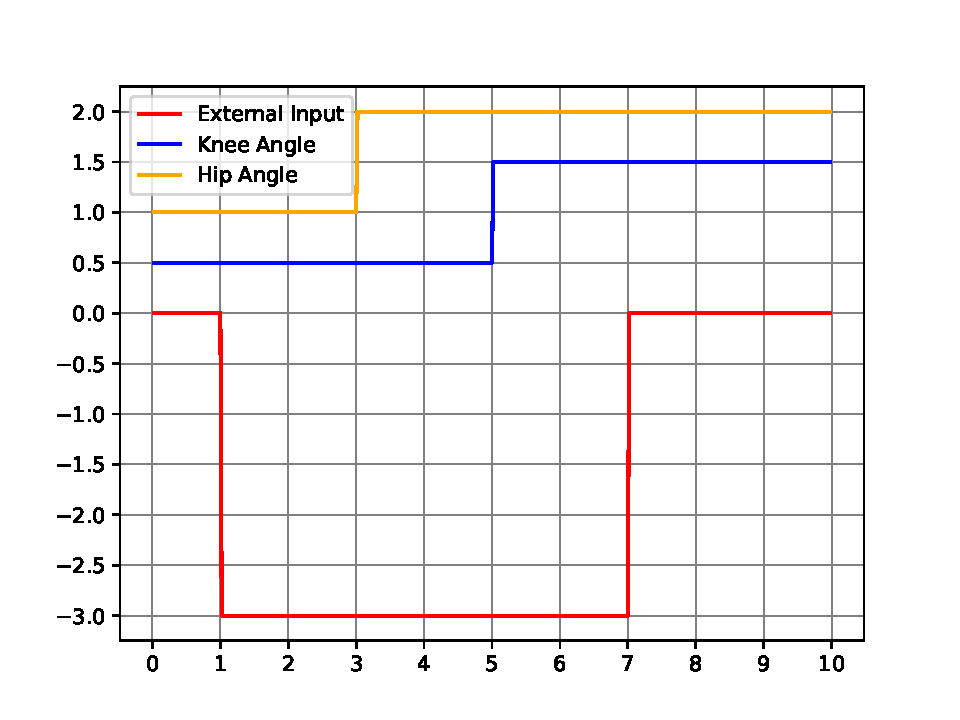
\includegraphics[width=.5\textwidth]{Test Input}
	\caption{Test input}
	\label{fig:Test input}
\end{figure}

As shown in the figure \ref{fig:Test input}, this test input data is selected to evaluate the performance of the controllers. External control input is applied at $t=1$ and is maintained until $t=7$ to see the response. Additionally, changing the knee and hip angles at $t=3$ and $t=5$ respectively to see the response of the controller to the change in the configuration.

%two figures of the step response of the internal input and zoomed in for the hip angle effect
\begin{figure}[h]
	\centering
	\begin{subfigure}[t]{0.45\textwidth}
		\centering
		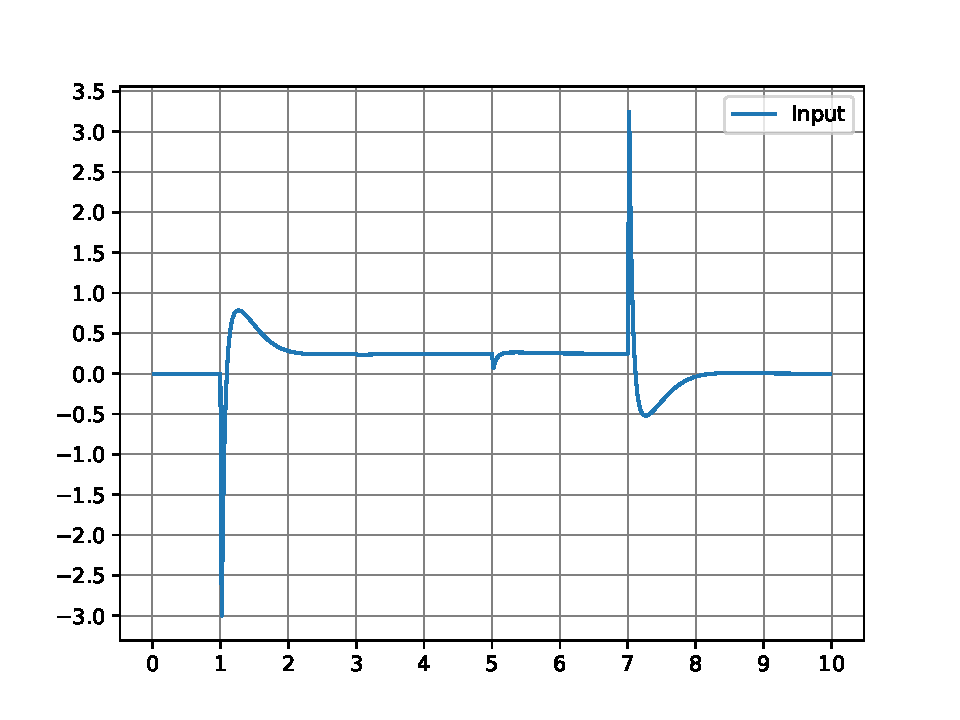
\includegraphics[width=\textwidth]{Step Response of the Internal Input}
		\caption{Step response of the internal input}
		\label{fig:Step response of the internal input}
	\end{subfigure}
	\begin{subfigure}[t]{0.45\textwidth}
		\centering
		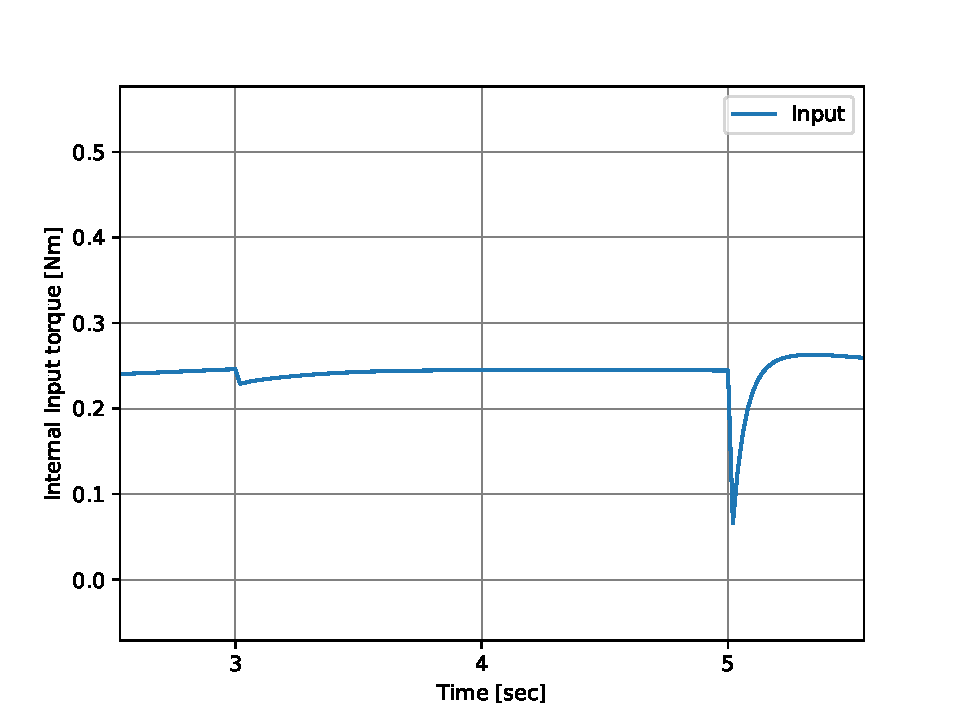
\includegraphics[width=\textwidth]{Step Response of the Internal Input hip angle}
		\caption{Step response of the hip and knee angles}
		\label{fig:Step response of the hip and knee angles}
	\end{subfigure}
	\caption{Step response of the internal input}
	\label{fig:Step response of the internal input}
\end{figure}
%%figure of the step response of the internal input
%\begin{figure}[h]
%	\centering
%	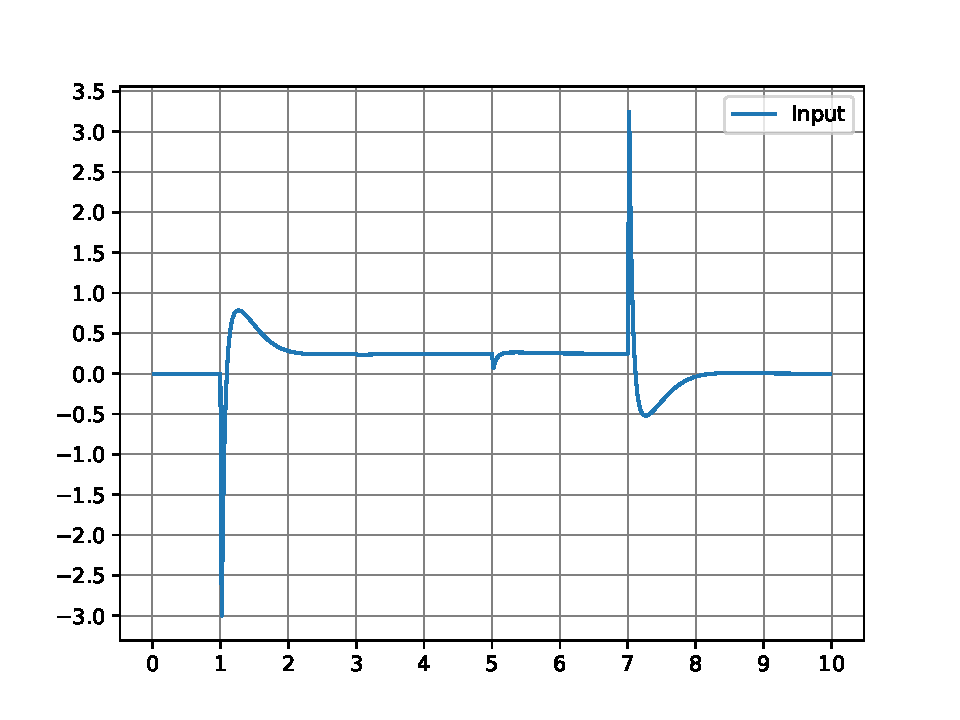
\includegraphics[width=.5\textwidth]{Step Response of the Internal Input}
%	\caption{Step response of the internal input}
%	\label{fig:Step response of the internal input}
%\end{figure}
The internal input is the input that is generated by the controller and is used to control the robot. The step response of the internal input is shown in the figure \ref{fig:Step response of the internal input}.The figure shows the response at time $t=1$ when the external input is applied where it overshoots and then converges to a value of $0.25$ which indicates that the robot is moving forward and the external input is still applied. The figure \ref{fig:Step response of the hip and knee angles} shows the response of the hip and knee angles to the change in the configuration at $t=3$ and $t=5$ respectively. The effect of the change in knee angle is more significant than the effect of the change in the hip angle since the knee angle has much higher effect on the center of gravity location than the hip angle.The stop of the external input is reflected in the response at $t=7$ where the internal input converges to $0$ which indicates that the robot is not moving forward anymore.
%two sub figures for the s and s dot
\begin{figure}[h]
	\centering
	\begin{subfigure}[t]{0.45\textwidth}
		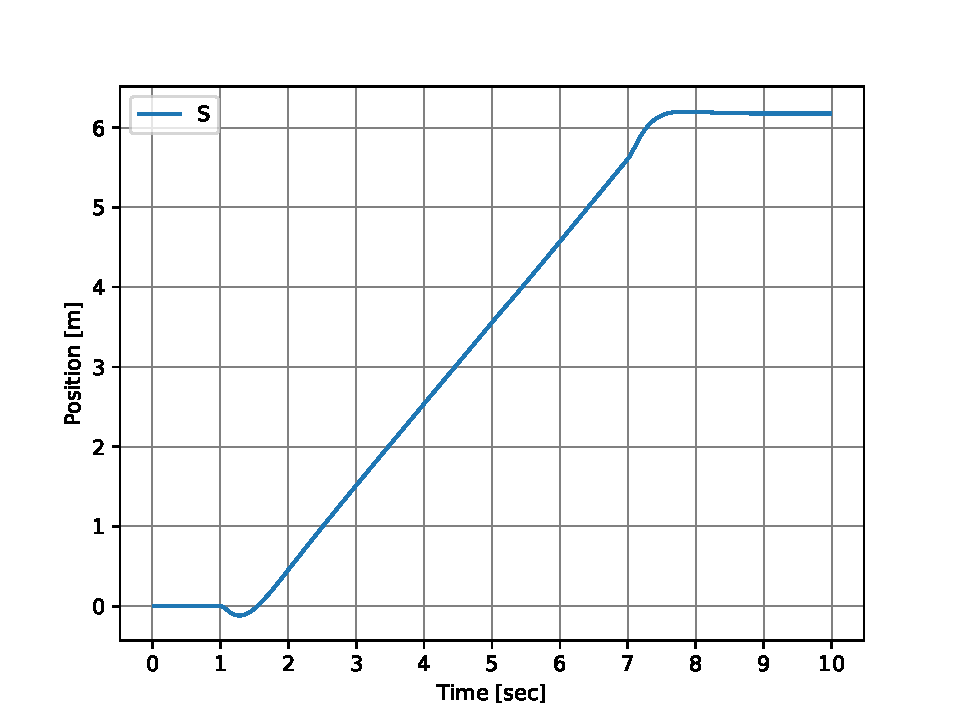
\includegraphics[width=\textwidth]{S}
		\caption{S}
		\label{fig:S}
	\end{subfigure}
	\begin{subfigure}[t]{0.45\textwidth}
		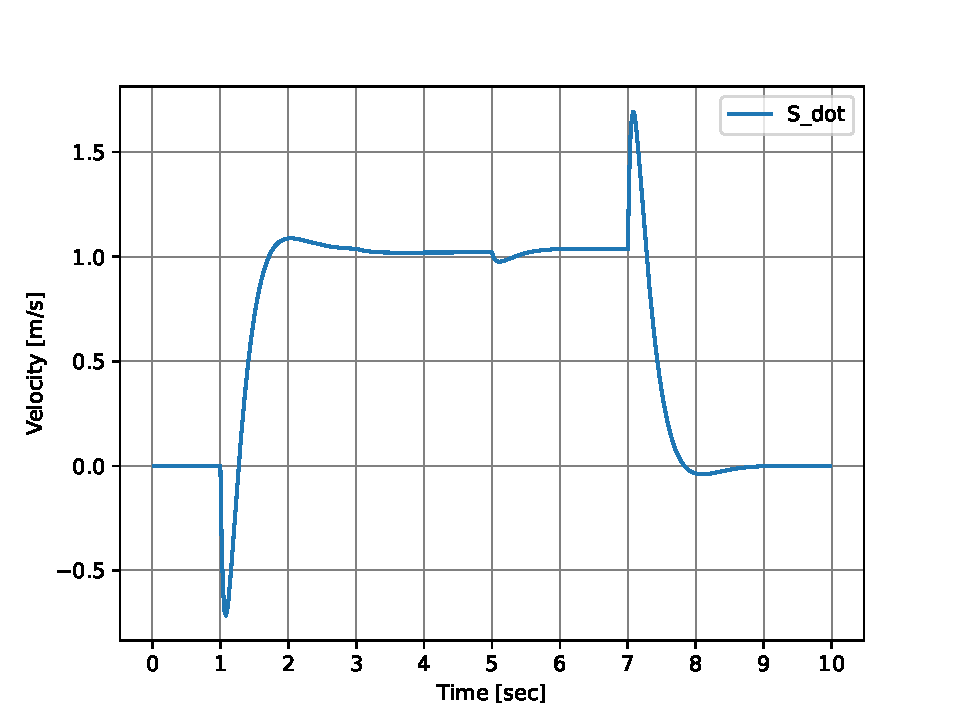
\includegraphics[width=\textwidth]{S_dot}
		\caption{S dot}
		\label{fig:S dot}
	\end{subfigure}
	\caption{S and S dot}
	\label{fig:S and S dot}
\end{figure}

As shown in the figure \ref{fig:S and S dot}, the s is the x position of the robot. The s dot is the derivative of the s. As showen in the figure \ref{fig:S} at $t=1$ the robot starts moving slightly backward befor it starts moving forward. The center of gravity is learned a bit forward with translates into a slightly backward movement.Afterwards the controller keeps the balance of the robot while it is moving forward.The external input is stopped at $t=7$ which is reflected in the figure \ref{fig:S} at $t=7$ where the robot comes to a stop. The figure \ref{fig:S dot} shows the velocity of the robot. The velocity is disrupted at $t=3$ and $t=5$ when the hip and knee angles are changed respectively.
% two sub figures for the theta and theta dot
\begin{figure}[h]
	\centering
	\begin{subfigure}[t]{0.45\textwidth}
		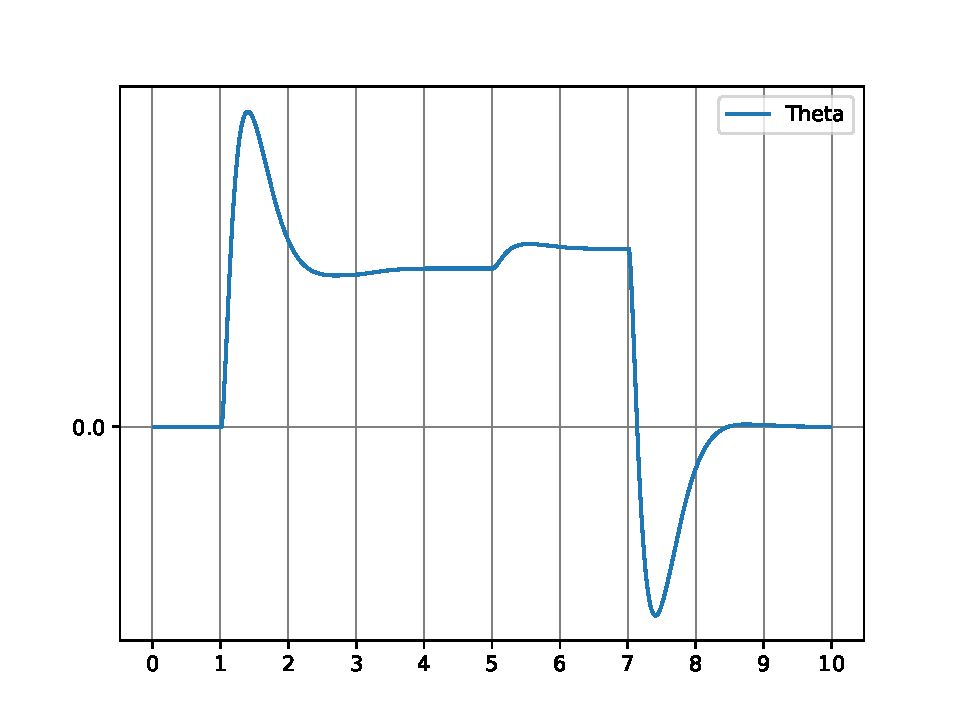
\includegraphics[width=\textwidth]{Theta}
		\caption{Theta}
		\label{fig:Theta}
	\end{subfigure}
	\begin{subfigure}[t]{0.45\textwidth}
		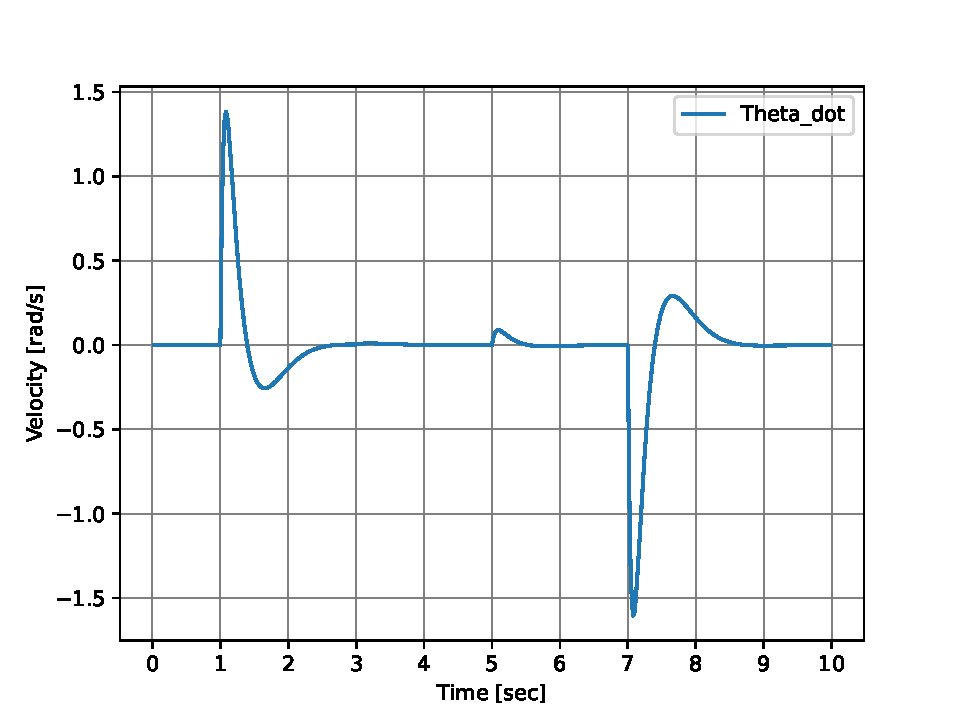
\includegraphics[width=\textwidth]{Theta_dot}
		\caption{Theta dot}
		\label{fig:Theta dot}
	\end{subfigure}
	\caption{Theta and Theta dot}
	\label{fig:Theta and Theta dot}
\end{figure}

As shown in the figure \ref{fig:Theta and Theta dot}, the theta is the angle between the center of gravity and the vertical axis to the ground. The theta dot is the derivative of the theta.
%two sub figures for the psi and psi dot
\begin{figure}[h]
	\centering
	\begin{subfigure}[t]{0.45\textwidth}
		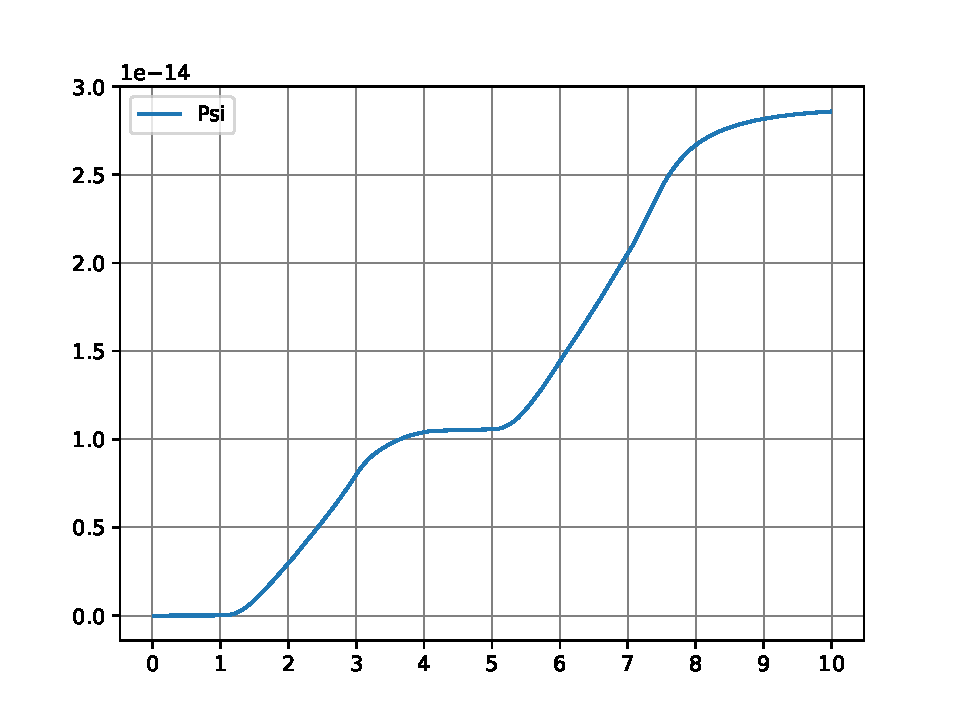
\includegraphics[width=\textwidth]{Psi}
		\caption{Psi}
		\label{fig:Psi}
	\end{subfigure}
	\begin{subfigure}[t]{0.45\textwidth}
		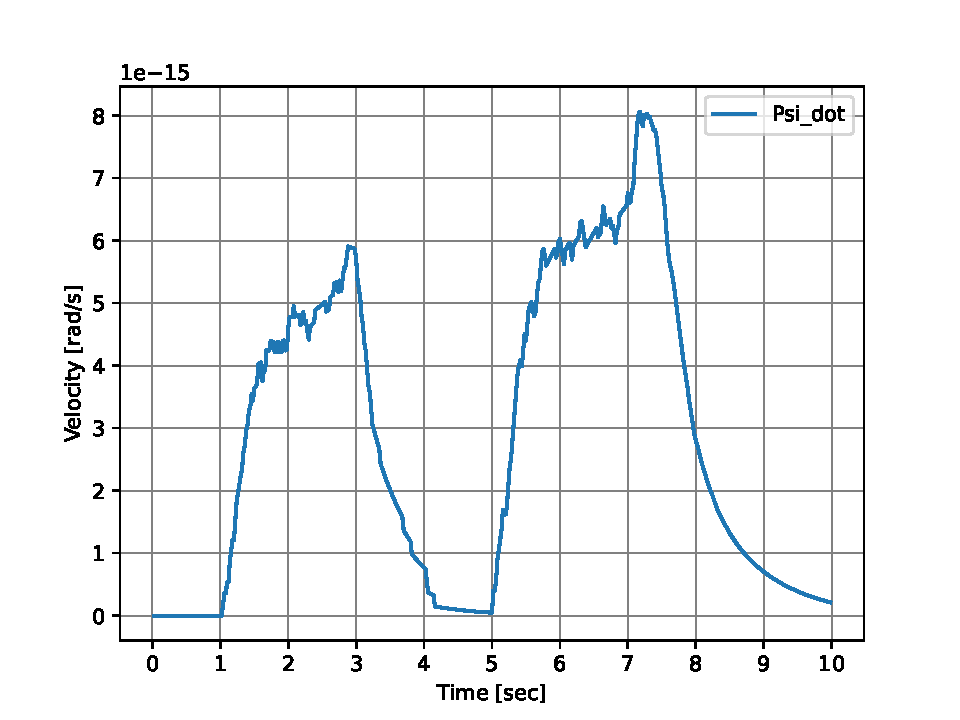
\includegraphics[width=\textwidth]{Psi_dot}
		\caption{Psi dot}
		\label{fig:Psi dot}
	\end{subfigure}
	\caption{Psi and Psi dot}
	\label{fig:Psi and Psi dot}
\end{figure}

As shown in the figure \ref{fig:Psi and Psi dot}, the %


%figure for the Gamma
\begin{figure}[h]
	\centering
	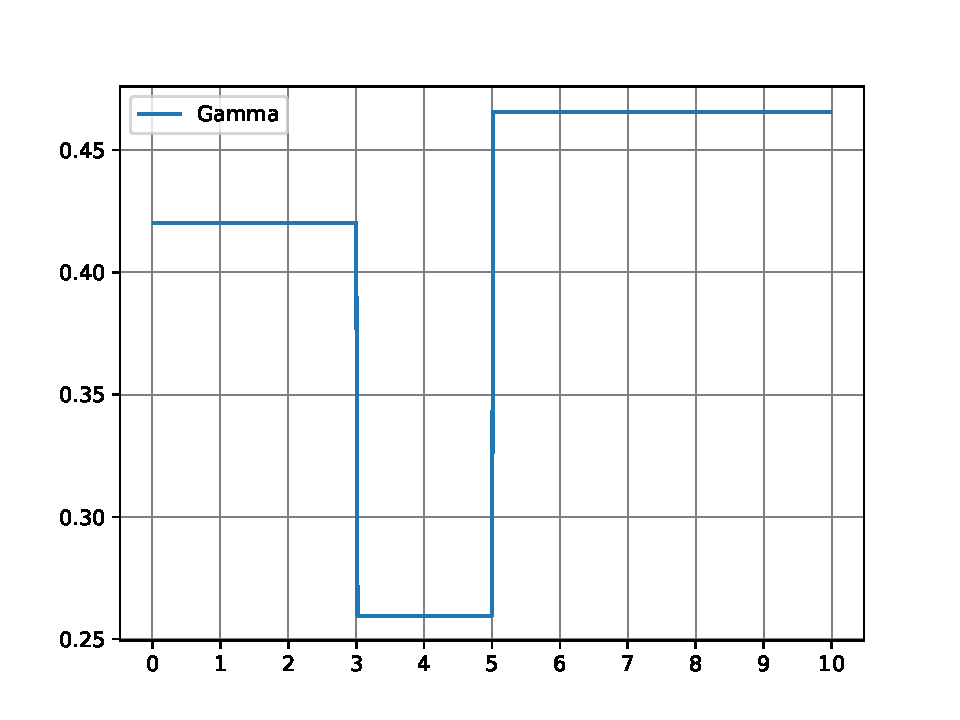
\includegraphics[width=.5\textwidth]{Gamma}
	\caption{Gamma}
	\label{fig:Gamma}
\end{figure}

The Gamma angle is the angle between the center of gravity and the link 1. As shown in the figure \ref{fig:Gamma}, the Gamma angle is changed at $t=3$ and $t=5$ when the hip and knee angles are changed respectively. It decreased to zero if the robot is verticallly aligned with the ground meaning when the hip and knee angles are zero.

%figure for L_m L_x L_b and L
\begin{figure}[h]
	\centering
	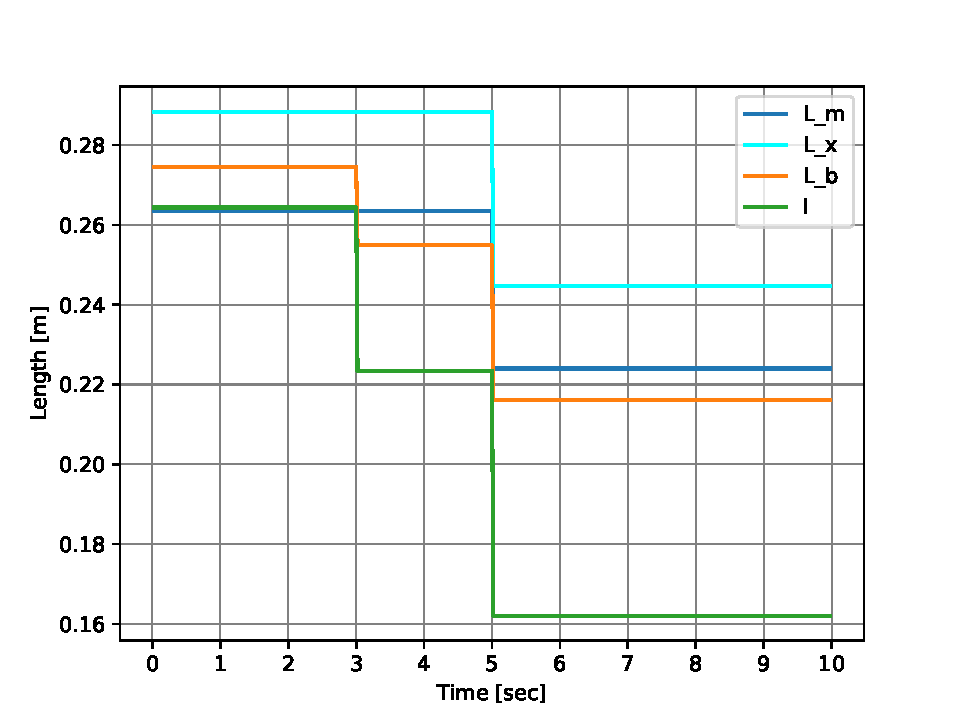
\includegraphics[width=.5\textwidth]{L_m L_x L_b L}
	\caption{Lm Lx Lb and L}
	\label{fig:Lm Lx Lb and L}
\end{figure}

As shown in the figure \ref{fig:Lm Lx Lb and L}, the Lm Lx Lb and L are changed at $t=3$ and $t=5$ when the hip and knee angles are changed respectively.
%figure for comparison between the two external inputs
\begin{figure}[h]
	\centering
	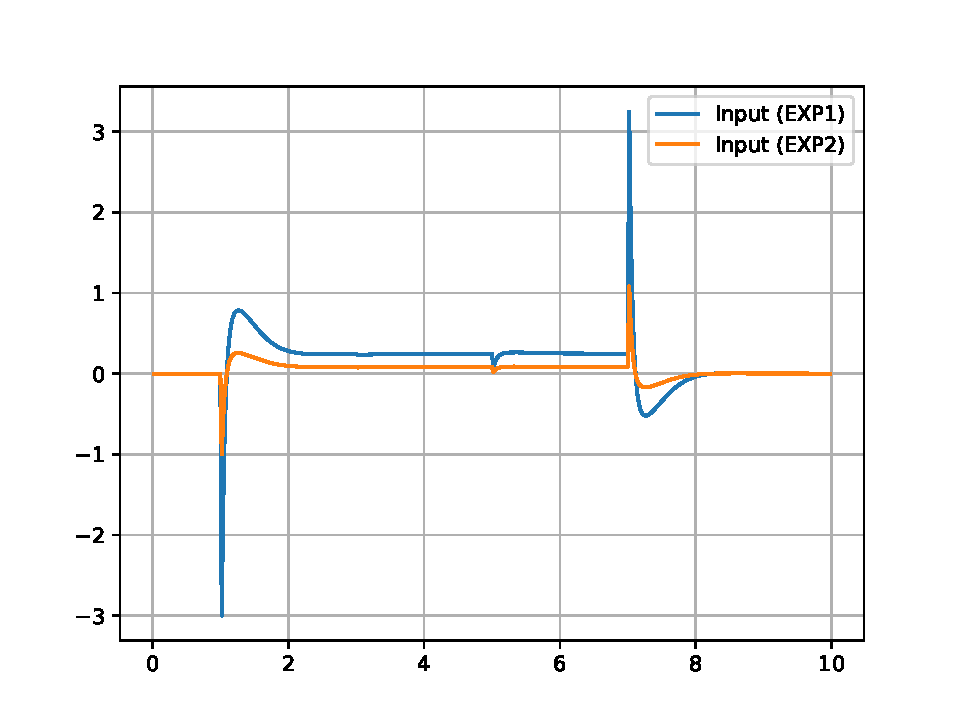
\includegraphics[width=.5\textwidth]{Comparison between the two external inputs}
	\caption{Comparison between the two external inputs}
	\label{fig:Comparison between the two external inputs}
\end{figure}

In the figure \ref{fig:Comparison between the two external inputs}, two different external inputs are applied to the robot. In experment 1, 1 unit of external input is applied to the robot. In experment 2, 3 units of external input is applied to the robot. The experment 2 shows a better response than experment 1.The overshoot is less and the robot converges to the desired state faster. In addition, the robot is more stable when the hip and knee angles are changed at $t=3$ and $t=5$ respectively.
%	\item \textbf{Impact of Non-Retuning:} Discussion on the effects of not retuning the controllers.
\subsection{Impact of Non-Retuning}

%	\item \textbf{Influence of Leg Configuration:} Analysis of how leg configuration influences the robot's behavior.
If the controller is not returned when the configuration changes, the old K gains that rely on the old center of gravity location will be used, resulting in a poor response.
\subsection{Influence of Leg Configuration}
%	\item \textbf{Controller Setting Comparisons:} Comparative study of different controller settings and a comparison between LQR and Pole-Placement controllers.
\subsection{Controller Setting Comparisons}
%	\item \textbf{Optimal Controller Configuration:} Conclusion on which controller configuration might be best suited for such a robot.
%\end{itemize}



%%pitch angle







	


